% $HeadURL$

\subsection{Glyph: \glyph{Multimer}}
\label{sec:multimer}

As its name implies, a multimer is an aggregation of multiple identical or pseudo-identical entities held together by non-covalent bonds (Thus, they are distinguished from polymers by the fact that the later involve covalent bonds). Here,  \emph{pseudo-identical} refers to the possibility that the entities differ chemically but retain some common global characteristic, such as a structure or function, and so can be considered identical within the context of the SBGN \PD.  An example of this are the homologous subunits in a hetero-oligomeric receptor. SBGN \PD accepts multimers of \glyph{simple chemical} (\sect{simpleChemical}), \glyph{macromolecule} (\sect{macromolecule}), \glyph{nucleic acid feature} (\sect{genetic}) or \glyph{complex} (\sect{complex}).

\begin{glyphDescription}

\glyphSboTerm %SBO:0000286 ! multimer
\begin{tabular}{l l}
Macromolecule & SBO:0000420 ! multimer of macromolecules \\
Complex & SBO:0000418 ! multimer of complexes \\
Nucleic Acid Feature & SBO:0000419 ! multimer of informational molecule segments \\
Simple Chemical & SBO:0000421 ! multimer of simple chemicals
\end{tabular}

\glyphContainer A \glyph{multimer} is represented by two identical containers shifted horizontally and vertically and stacked one on top of the other.  \fig{multimer} illustrates the glyph.

\glyphLabel A \glyph{multimer} has no identity on its own.  However, the first of the monomers carries an identifying label.  The label is placed in an unbordered box containing a string of characters.  The characters can be distributed on several lines to improve readability, although this is not mandatory.  The label box must be attached to the center of the top monomer's container.  The label may spill outside of the container.

\glyphAux A \glyph{multimer} can carry state variables that can add information about its state (\sect{stateVariable}).  The state of a multimer is therefore defined as the vector of all its state variables.  Note that a \glyph{state variable} carried by a multimer actually applies to each of the constituent monomers individually.  If instead the state variables are meant to apply to the whole multimeric assembly, a \glyph{macromolecule} (\sect{macromolecule}) should be used instead of \glyph{multimer}.  An assembly containing some state variables applicable to the components, and others state variable applicable to the assembly (for instance opening of a channel and phosphorylation of each of its subunits) should be represented by a \glyph{complex} (\sect{complex}).

A \glyph{multimer} can also carry one or several \glyph{units of information} (\sect{unitInfo}).  The information can characterize a domain, such as a binding site.  Particular \glyph{units of information} exist for describing the material type (\sect{material-types-cv}), the conceptual type (\sect{conceptual-types-cv}), and the cardinality (\sect{cardinality-cv}) of the multimer.  Note that a \glyph{unit of information} carried by a multimer actually applies to each of the constituent monomers individually.  If instead a \glyph{unit of information} should be applicable to the whole multimeric assembly, a \glyph{macromolecule} should be used (\sect{macromolecule}). An assembly containing units of information applying to the components, and others to the assembly should be represented by a \glyph{complex} (\sect{complex}).

A \glyph{multimer} may also carry a \glyph{clone marker} (\sect{cloneMarker}).

\end{glyphDescription}


\begin{figure}[H]
  \centering
  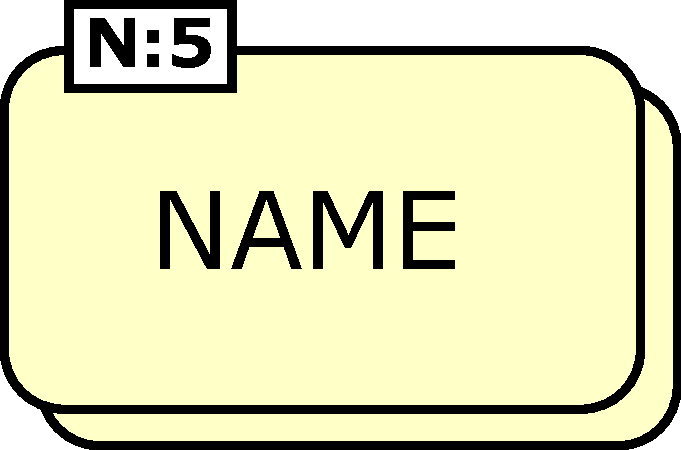
\includegraphics[scale = 0.3]{images/multimer}
  \caption{The \PD glyph for \glyph{multimer} with an additional unit of information containing the cardinality.}
  \label{fig:multimer}
\end{figure}






% The following is for [X]Emacs users.  Please leave in place.
% Local Variables:
% TeX-master: "../sbgn_PD-level1"
% End:
